\documentclass{article}
\usepackage{graphicx}
\usepackage{hyperref}
\usepackage{caption}

\hypersetup{
    colorlinks=false,
    pdfborderstyle={/S/U/W 0} % 默认无边框
}

% 定义一个用于图表引用的命令,仅为引用添加红色边框
\newcommand{\figureref}[1]{%
    \begingroup
    \hypersetup{pdfborderstyle={/S/S/W 1}, linkbordercolor={1 0 0}} % 方框样式,红色
    \ref{#1}%
    \endgroup
}

\captionsetup[figure]{name=图, labelsep=colon}

\begin{document}

\subsection{图表的创建和引用}
The above data is combined to form a correlation heat map between features, as shown in Fig.\figureref{fig:time-freq}
\begin{figure}[h]
    \centering
    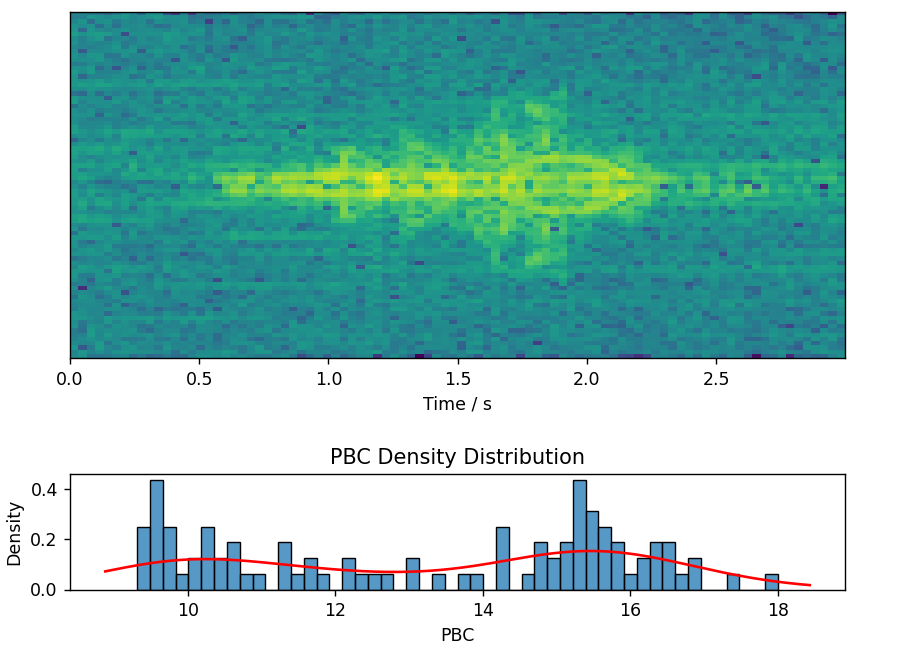
\includegraphics[width=1\textwidth]{时频图和PBC分布图.png}
    \caption{时频图和PBC分布图}
    \label{fig:time-freq}
\end{figure}

\end{document}
